% !TeX program = xelatex
\documentclass[UTF8]{beamer}

% -----------------------------------------------------------------------------
% Language, typography, mathematics, tables, graphics
% -----------------------------------------------------------------------------
\usepackage{xeCJK}
\usepackage{amsmath}
\usepackage{physics}
\usepackage{booktabs}
\usepackage{tabularx}
\usepackage{array}
\usepackage{graphicx}
\usepackage{xcolor}
\usepackage{tcolorbox}
\usepackage{url}
\urlstyle{tt}
\tcbuselibrary{skins}
\usepackage{tikz}
\usetikzlibrary{arrows.meta,positioning,calc}

% Preserve the reusable presentation typography.
\usepackage[T1]{fontenc}
\usepackage{palatino}
\setCJKmainfont{Noto Serif CJK SC}
\setCJKsansfont{Noto Serif CJK SC}
\setCJKmonofont{Noto Serif CJK SC}
\setmonofont{Inconsolata}
\def\mathfamilydefault{\rmdefault}

% 16:9 slide canvas from the Durham/Stanford template.
\usepackage[
  orientation=landscape,
  size=custom,
  width=16,
  height=9,
  scale=0.5
]{beamerposter}

% Compatibility fix for older Babel releases.
\makeatletter
\let\@@magyar@captionfix\relax
\makeatother

% -----------------------------------------------------------------------------
% Theme and deck-specific visual language
% -----------------------------------------------------------------------------
\usetheme{Stanford}
\beamertemplatenavigationsymbolsempty
\setbeamerfont{frametitle}{size=\Large,series=\bfseries}
\setbeamerfont{title}{size=\LARGE,series=\bfseries}
\setbeamercolor{itemize item}{fg=darkcyan}
\setbeamercolor{itemize subitem}{fg=darkcyan}
\setbeamercolor{enumerate item}{fg=darkcyan}

\definecolor{planblue}{RGB}{29,78,121}
\definecolor{planteal}{RGB}{0,124,146}
\definecolor{plangreen}{RGB}{0,128,96}
\definecolor{plangold}{RGB}{188,122,25}
\definecolor{planrose}{RGB}{174,63,79}
\definecolor{planred}{RGB}{158,42,43}
\definecolor{planpale}{RGB}{244,247,249}

\newtcolorbox{phasebox}[2][]{%
  enhanced,
  colback=white,
  colframe=#2,
  boxrule=1.2pt,
  arc=1.5mm,
  left=1.6mm,
  right=1.6mm,
  top=0.9mm,
  bottom=0.9mm,
  before upper={\raggedright},
  #1
}

\newcommand{\metric}[3]{%
  \begin{tcolorbox}[
    enhanced,
    colback=#1!7,
    colframe=#1,
    boxrule=1.0pt,
    arc=1.2mm,
    left=1.8mm,
    right=1.8mm,
    top=0.5mm,
    bottom=0.5mm,
    before upper={\raggedright}
  ]
    {\color{#1}\bfseries\large #2}\hspace{1.0ex}{\footnotesize #3}
  \end{tcolorbox}%
}

\newcommand{\source}[1]{%
  \par\vfill\nointerlineskip
  \hbox to \linewidth{\hfill
    \smash{\raisebox{0pt}[0pt][0pt]{\tiny\color{coolgray}Source: #1}}}%
}

\newcommand{\Mpch}{\,h^{-1}\mathrm{Mpc}}

% -----------------------------------------------------------------------------
% Presentation metadata
% -----------------------------------------------------------------------------
\title[DEGRACE ECOSMOG suite]{\textbf{The DEGRACE ECOSMOG suite}}
\subtitle{What is on disk, what is pinned, and what MG-GLAM companions need}

\author[C.-Z. Ruan]{\Large Cheng-Zong Ruan}

\institute[Durham University]{%
  
\includegraphics[height=0.72in]{durham_logo.png}\\[0.65ex]
  \small Institute for Computational Cosmology, Durham University
}
\date{17 October 2026 \quad\textcolor{coolgray}{\small survey of Baojiu Li's runs, 16 Oct 2026}}

% -----------------------------------------------------------------------------
% Document
% -----------------------------------------------------------------------------
\begin{document}

\begin{frame}[plain]
  \titlepage
\end{frame}

% -----------------------------------------------------------------------------
\begin{frame}{Executive summary}
  \footnotesize
  \begin{columns}[T,totalwidth=\textwidth]
    \begin{column}{0.56\textwidth}
      \begin{phasebox}[colback=plangreen!6,top=1.0mm,bottom=1.0mm]{plangreen}
        {\color{plangreen}\bfseries Pinned from the files on disk}\par\smallskip
        \scriptsize
        \begin{itemize}\setlength\itemsep{0.2em}
          \item 96 nodes of a Sobol design in $(\Omega_m, h, S_8, n_s, \log_{10}|f_{R0}|)$; every derived parameter reproduced exactly.
          \item f(R) (cosma7) and $\Lambda$CDM (cosma8) twins from the \emph{same} 2LPTic ICs; seed 2026 for all nodes.
          \item 43 outputs per run: 17 primary $z$ + 25 stations at $\chi = 256\,k\Mpch$ in each node's own background, verified to $2\times10^{-7}$.
          \item All 192 runs reach $a = 1$; Gadget snapshots and f(R) $P(k)$ at every epoch.
        \end{itemize}
      \end{phasebox}
      \vspace{0.4ex}
      \begin{phasebox}[colback=planred!5,top=1.0mm,bottom=1.0mm]{planred}
        {\color{planred}\bfseries Two things to raise with Baojiu}\par\smallskip
        \scriptsize
        \begin{itemize}\setlength\itemsep{0.2em}
          \item CAMB was fed $\omega_c = \Omega_m h^2$: linear spectra have $\Omega_m^{\rm CAMB} = \Omega_m + \Omega_b + \Omega_\nu$, 0.04--0.055 too high.
          \item Nodes 1--80 carry two byte-different Gadget conversions (15 and 27 March).
        \end{itemize}
      \end{phasebox}
    \end{column}
    \hfill
    \begin{column}{0.41\textwidth}
      \metric{planblue}{96}{nodes, $1024^3$ in $1024\Mpch$, $z_{\rm init}=49$}
      \metric{planteal}{192}{complete runs (f(R) + $\Lambda$CDM twins)}
      \metric{plangold}{43}{outputs per run, per-node epoch lists}
      \metric{plangreen}{0}{consistency failures over 96 nodes}
      \vspace{0.3ex}
      \begin{phasebox}[colback=planpale,top=0.8mm,bottom=0.8mm]{planblue}
        \scriptsize
        Reference: \texttt{docs/degrace\_ecosmog/} (README, \texttt{nodes.csv}, \texttt{aout.json}, extraction script).
      \end{phasebox}
    \end{column}
  \end{columns}
  \source{bl267 directories on cosma7 (dp004) and cosma8 (dp203), read 2026-10-16}
\end{frame}

% -----------------------------------------------------------------------------
\begin{frame}{Where everything lives}
  \scriptsize
  \texttt{C7} $=$ \path{/cosma7/data/dp004/bl267/Runs/DEGRACE} \quad
  \texttt{C8} $=$ \path{/cosma8/data/dp203/bl267/Projects/Ongoing/DEGRACE}
  \par\smallskip
  \setlength{\tabcolsep}{4pt}
  \begin{tabular}{@{}l>{\ttfamily}p{0.5\textwidth}>{\raggedright\arraybackslash}p{0.27\textwidth}@{}}
    \toprule
    item & \normalfont path & notes \\
    \midrule
    design, generators, CAMB & C7/ICs/CAMB/Parameter\_files/Python\_codes/ & \texttt{DEGRACE\_L512.csv}, \texttt{Run\_CAMB.py}, \texttt{Run\_2LPTic.py}, \texttt{Gen\_ECOSMOG\_Params.py}, \texttt{params\_nXXX.ini} \\
    initial conditions & C8/ICs/IC\_data/L1024/Node\_XXX/ics.0..27 & 30\,GB per node; CAMB $P(k)$ and 2LPTic logs beside them \\
    $\Lambda$CDM runs & C8/Runs/LCDM/Node\_XXX/ & namelist, info files, \texttt{gadget\_data} \\
    f(R) runs & C7/Runs/L1024/FR/Node\_XXX/ & same layout, restarts \\
    f(R) $P(k)$ & C7/Runs/L1024/FR/power\_spectra/Node\_XXX/ & POWMES, 43 epochs \\
    fiducial node & C7/Runs/L1024/FR/Node\_900/ & Planck ($\Omega_m$ 0.3089, $h$ 0.6774); job script only, no ICs \\
    tests & C8/Runs/L512/Node\_002, C8/Runs/L256 & node-2 cosmology, $\Lambda$CDM + f(R) \\
    not run & C7/Runs/L1024/GR/Np2048/Node\_002 & ICs \texttt{L1024h} never generated \\
    obsolete & C8/ICs/IC\_data/L1024\_old/ & earlier design (101 nodes): do not use \\
    \bottomrule
  \end{tabular}

  \vspace{1ex}
  \begin{phasebox}[colback=planpale,top=0.8mm,bottom=0.8mm]{plangold}
    Nodes 097--100 are empty $\Lambda$CDM run directories (namelist only); the generators loop over 1--96. The suite is 96 nodes.
    Raw RAMSES particle files were deleted after conversion: only \texttt{info\_000NN.txt} remains per output.
  \end{phasebox}
\end{frame}

% -----------------------------------------------------------------------------
\begin{frame}{The design: a Sobol sequence in five parameters}
  \footnotesize
  \begin{columns}[T,totalwidth=\textwidth]
    \begin{column}{0.46\textwidth}
      \scriptsize
      \setlength{\tabcolsep}{4pt}
      \begin{tabular}{@{}clc@{}}
        \toprule
        col & parameter & range (nodes 1--96) \\
        \midrule
        1 & $\Omega_m$ & 0.25 -- 0.349 \\
        2 & $h$ & 0.65 -- 0.749 \\
        3 & $S_8$ & 0.65 -- 0.945 \\
        4 & $n_s$ & 0.90 -- 1.049 \\
        5 & $\log_{10}|f_{R0}|$ & $-6.5$ -- $-4.02$ \\
        6 & unused & $-0.45$ -- $0.98$ \\
        7--12 & unit-cube coordinates & \\
        \bottomrule
      \end{tabular}
      \vspace{0.8ex}
      \begin{phasebox}{planblue}
        {\color{planblue}\bfseries Derived, verified for all 96 nodes}\par\smallskip
        \scriptsize
        $\Omega_b = 0.02237/h^2$, flat, $\Omega_\Lambda = 1 - \Omega_m$\\
        $\sigma_8 = S_8\sqrt{0.3/\Omega_m}$ (ICs within $10^{-4}$: CAMB $A_s$ tuning tolerance)\\
        $f_{R0} = -10^{\rm col\,5}$, Hu--Sawicki $n = 1$\\
        ECOSMOG \texttt{fr\_c1oc22} $= |f_{R0}|\,(12/\Omega_m - 9)^2$ (to $10^{-9}$)\\
        \texttt{dens\_V\_on} = 80 / 120 / 160 for $|f_{R0}| < 10^{-6}$ / $< 10^{-5}$ / else
      \end{phasebox}
    \end{column}
    \hfill
    \begin{column}{0.52\textwidth}
      \centering
      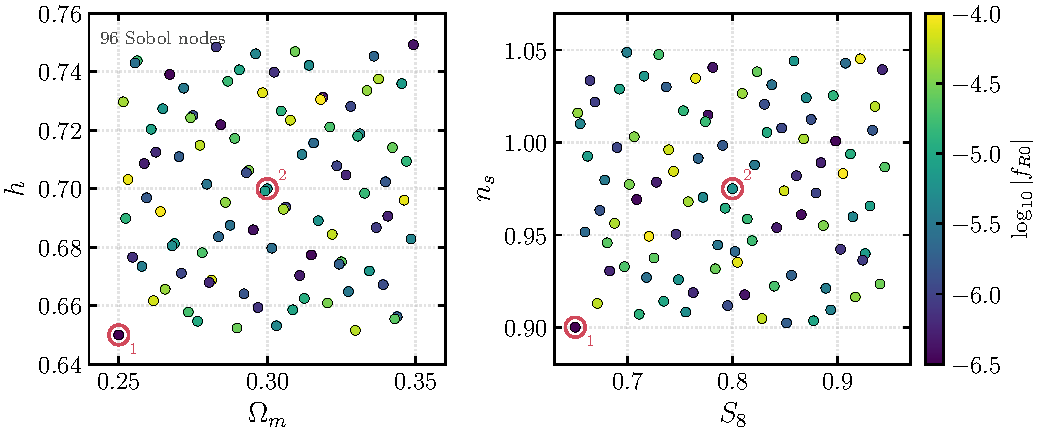
\includegraphics[width=\linewidth]{figs/design_coverage.pdf}
      \par\scriptsize Node 1 is the lower corner of every range, node 2 the centre; colour is $\log_{10}|f_{R0}|$.
    \end{column}
  \end{columns}
  \source{\texttt{DEGRACE\_L512.csv} (512 rows); \texttt{figs/make\_suite\_fig.py}}
\end{frame}

% -----------------------------------------------------------------------------
\begin{frame}{Initial conditions: 2LPTic, seed 2026 for every node}
  \footnotesize
  \begin{columns}[T,totalwidth=\textwidth]
    \begin{column}{0.5\textwidth}
      \scriptsize
      \setlength{\tabcolsep}{3pt}
      \begin{tabular}{@{}ll@{}}
        \toprule
        setting & value \\
        \midrule
        box, particles & $1024\Mpch$, $1024^3$ (\texttt{Nmesh} 1024) \\
        glass & one-particle glass tiled $1024\times$: regular grid \\
        start & $z = 49$, second-order LPT \\
        seed & \textbf{2026 for every node} \\
        spectrum & CAMB $z{=}0$ table as $(\log_{10}k,\ \log_{10}4\pi k^3P)$ \\
        normalisation & rescaled to \texttt{Sigma8} (\texttt{Normfac} in the log) \\
        tilt & \texttt{PrimordialIndex = 1} (none beyond CAMB's $n_s$) \\
        units & Mpc/h, $10^{10}\,M_\odot/h$, km/s \\
        files & Gadget-1, little-endian, 28 files, 30\,GB per node \\
        growth factor & \texttt{inputspec\_ics.txt} line 1: $(49,\ D_+ \text{ ratio})$ \\
        \bottomrule
      \end{tabular}
    \end{column}
    \hfill
    \begin{column}{0.47\textwidth}
      \begin{phasebox}[colback=plangreen!6]{plangreen}
        {\color{plangreen}\bfseries Why this matters for companions}\par\smallskip
        \scriptsize
        \begin{itemize}\setlength\itemsep{0.2em}
          \item f(R) and $\Lambda$CDM of a node share the same IC files: matched-phase twins.
          \item Fixed seed across the design: cosmology dependence is not confused with sample variance.
          \item MG-GLAM can ingest the identical files with \texttt{ic2pm} (default \texttt{half} velocity epoch), giving a third matched run.
        \end{itemize}
      \end{phasebox}
      \vspace{0.4ex}
      \begin{phasebox}{planteal}
        {\color{planteal}\bfseries Checks on disk}\par\smallskip
        \scriptsize
        RAMSES \texttt{info} headers ($H_0$, $\Omega_m$, $\Omega_\Lambda$) agree with \texttt{2LPTic.param} for all nodes;
        Gadget header: Box 1024, $a = 0.02$, $1024^3$, mass 6.94 (node 1). POWMES $P(k)$ of every IC set at $z = 49$ (\texttt{PK\_LCDM\_NXXX\_S01.dat}).
      \end{phasebox}
    \end{column}
  \end{columns}
  \source{\texttt{2LPTic.param}, \texttt{log\_2LPTic.txt}, \texttt{Run\_2LPTic.py}}
\end{frame}

% -----------------------------------------------------------------------------
\begin{frame}{Linear spectra: CAMB settings and the $\omega_c$ pitfall}
  \footnotesize
  \begin{columns}[T,totalwidth=\textwidth]
    \begin{column}{0.47\textwidth}
      \begin{phasebox}{planblue}
        {\color{planblue}\bfseries Template (Planck 2018 base), per-node overrides}\par\smallskip
        \scriptsize
        $\omega_b = 0.02237$, $\omega_\nu = 0.0006442$ (one 0.06\,eV neutrino, $N_{\rm eff}=3.046$),
        $\Omega_k = 0$, $w = -1$, $\tau = 0.0544$, $T_{\rm CMB} = 2.7255$, $Y_{\rm He} = 0.24$,
        pivot 0.05\,Mpc$^{-1}$, no running, $k_{\max} = 20$, 5 per log-int, linear, $z = 0$ only.\par\smallskip
        Per node: \texttt{hubble}, \texttt{omch2}, $n_s$; $A_s$ iterated until $\sigma_8(z{=}0)$ hits
        $S_8\sqrt{0.3/\Omega_m}$ within $10^{-4}$.
      \end{phasebox}
      \vspace{0.4ex}
      \begin{phasebox}{plangold}
        {\color{plangold}\bfseries Files}\par\smallskip
        \scriptsize
        \texttt{PK\_CAMB\_z00\_XXX.dat}: $k/h$, $P(k)\,[(\mathrm{Mpc}/h)^3]$, 617 rows, $z = 0$. The copy beside the ICs is byte-identical to the cosma7 original.
      \end{phasebox}
    \end{column}
    \hfill
    \begin{column}{0.5\textwidth}
      \begin{phasebox}[colback=planred!5]{planred}
        {\color{planred}\bfseries Pitfall in \texttt{Run\_CAMB.py}}\par\smallskip
        \scriptsize
        The script computes \texttt{Oc = Om - Ob} but writes \texttt{omch2 = Om*h0**2}. CAMB's total matter is therefore
        \[
          \Omega_m^{\rm CAMB} = \Omega_m + \Omega_b + \Omega_\nu = \Omega_m + (0.041 \ldots 0.055),
        \]
        while 2LPTic, ECOSMOG and the $D_+$ scaling to $z = 49$ use the design $\Omega_m$. The \emph{shape} of
        every linear spectrum belongs to a higher $\omega_m$; the \emph{amplitude} is still the design $\sigma_8$
        because 2LPTic renormalises.\par\smallskip
        Harmless for companions that ingest the same ICs. Not harmless for emulator labels, ``linear'' ratios
        or halo-model inputs built from these files. \texttt{nodes.csv} carries both $\Omega_m$ values.
      \end{phasebox}
    \end{column}
  \end{columns}
  \source{\texttt{Run\_CAMB.py} lines 108--112; \texttt{params\_n001.ini}: omch2 = 0.10563 = $0.25 \times 0.65^2$}
\end{frame}

% -----------------------------------------------------------------------------
\begin{frame}{ECOSMOG configuration and run status}
  \footnotesize
  \begin{columns}[T,totalwidth=\textwidth]
    \begin{column}{0.55\textwidth}
      \scriptsize
      \setlength{\tabcolsep}{3pt}
      \begin{tabular}{@{}l>{\raggedright\arraybackslash}p{0.36\textwidth}@{}}
        \toprule
        namelist item & value \\
        \midrule
        \texttt{levelmin/levelmax} & 10 / 18: $1024^3$ root grid, 8 refinements, 3.9\,kpc/h finest cell \\
        \texttt{m\_refine} & 4,4,4,8,\ldots; \texttt{nsubcycle} 1,2,2,\ldots; \texttt{nremap} 10 \\
        \texttt{ngridtot/nparttot} & $3\times10^9$ / $1.5\times10^9$ \\
        cosmology & from the Gadget IC header \\
        $\Lambda$CDM twin & same namelist, \texttt{extradof=.false.} \\
        job & 560 MPI ranks, full nodes, 72\,h, restarts \\
        \bottomrule
      \end{tabular}
      \vspace{0.8ex}
      \begin{phasebox}[colback=plangreen!6]{plangreen}
        {\color{plangreen}\bfseries Status}\par\smallskip
        \scriptsize
        96/96 $\Lambda$CDM (cosma8, dp203) and 96/96 f(R) (cosma7, dp004) have all 43 outputs and end at $a = 1$.
      \end{phasebox}
    \end{column}
    \hfill
    \begin{column}{0.42\textwidth}
      \begin{phasebox}{planteal}
        {\color{planteal}\bfseries Extras found}\par\smallskip
        \scriptsize
        \begin{itemize}\setlength\itemsep{0.2em}
          \item \textbf{Node\_900}, the Planck fiducial ($\Omega_m$ 0.3089, $h$ 0.6774, $\Omega_b$ 0.0486): directory and job script
                created 8 Oct 2026, no ICs, not run. Its output list is the Slack list.
          \item \textbf{L512 node 2}: $\Lambda$CDM and f(R) test runs, 43 outputs each; \textbf{L256} $\Lambda$CDM test.
          \item \textbf{GR/Np2048 node 2}: $2048^3$ $\Lambda$CDM namelist prepared, ICs never generated.
          \item \textbf{L1024\_old}: 101 IC sets of an earlier design (node 1: $\Omega_m$ 0.333, $h$ 0.731). Superseded.
        \end{itemize}
      \end{phasebox}
    \end{column}
  \end{columns}
  \source{\texttt{namelist/cosmo.nml}, \texttt{run\_cosma8.bash}, \texttt{info\_000NN.txt}}
\end{frame}

% -----------------------------------------------------------------------------
\begin{frame}{Output epochs: the Slack convention, per node}
  \footnotesize
  \begin{columns}[T,totalwidth=\textwidth]
    \begin{column}{0.5\textwidth}
      \centering
      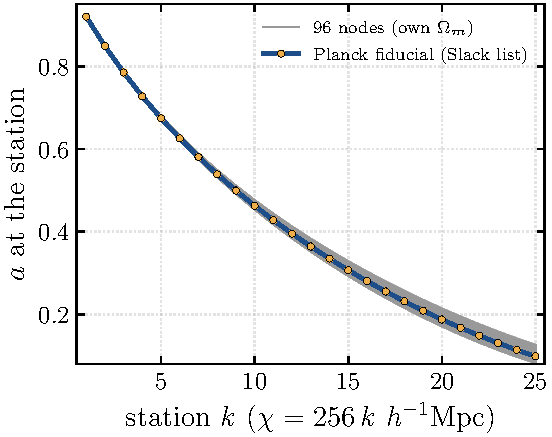
\includegraphics[width=0.92\linewidth]{figs/station_epochs.pdf}
    \end{column}
    \hfill
    \begin{column}{0.47\textwidth}
      \begin{phasebox}{planblue}
        {\color{planblue}\bfseries Generator (\texttt{Gen\_ECOSMOG\_Params.py})}\par\smallskip
        \scriptsize
        43 outputs = \texttt{output\_00001} at $a = 0.02$ plus 42 \texttt{aout}: $z = 0.125 \ldots 2.0$, $a = 1$, and the 25 roots
        of $\chi(a) = 256\,k\Mpch$, with $c/H_0 = 2997.92458\Mpch$ and $E^2 = \Omega_m a^{-3} + 1 - \Omega_m$
        (the node's own $\Omega_m$; matter and $\Lambda$ only).
      \end{phasebox}
      \vspace{0.3ex}
      \begin{phasebox}[colback=plangreen!6]{plangreen}
        {\color{plangreen}\bfseries Verified}\par\smallskip
        \scriptsize
        Recomputing the stations reproduces all $96 \times 25$ values to $2.3\times10^{-7}$ in $a$; 17 primary + 25 secondary in every list;
        f(R) and $\Lambda$CDM namelists carry identical lists.
      \end{phasebox}
      \vspace{0.3ex}
      \begin{phasebox}[colback=planpale]{plangold}
        \scriptsize
        Every node has 1--4 neighbouring targets closer than 0.5\,\% in $a$: the exact-$z$ scheduler accepts them since \texttt{cz}
        \texttt{ae4fa9d}. ECOSMOG itself dumps at the first step past each target, so actual snapshot epochs carry small offsets.
      \end{phasebox}
    \end{column}
  \end{columns}
  \source{\texttt{aout.json}; grey: 96 nodes, blue/gold: Planck fiducial list from Slack}
\end{frame}

% -----------------------------------------------------------------------------
\begin{frame}{Snapshot products}
  \footnotesize
  \begin{columns}[T,totalwidth=\textwidth]
    \begin{column}{0.5\textwidth}
      \begin{phasebox}{planblue}
        {\color{planblue}\bfseries Gadget conversions (r2g)}\par\smallskip
        \scriptsize
        \texttt{gadget\_data/output\_000NN/gadget.0 \ldots gadget.559}, one file per rank, with \texttt{r2g.config.snap\_NN} and a log.
        Little-endian Gadget-1, positions in \textbf{kpc/h} (BoxSize 1023999.98), masses $6.94\times10^{10}\,M_\odot/h$, IDs $1 \ldots 1024^3$.
        26--29\,GB per snapshot, about 1.2\,TB per node and gravity model.
      \end{phasebox}
      \vspace{0.3ex}
      \begin{phasebox}[colback=planred!5]{planred}
        {\color{planred}\bfseries Two conversions}\par\smallskip
        \scriptsize
        Nodes 001--080 also have \texttt{gadget\_data\_old} (15 March; the 27 March files are byte-different).
        Nodes 081--096 were converted once, later. Use \texttt{gadget\_data}; ask what changed in r2g.
      \end{phasebox}
    \end{column}
    \hfill
    \begin{column}{0.47\textwidth}
      \begin{phasebox}{plangold}
        {\color{plangold}\bfseries Power spectra}\par\smallskip
        \scriptsize
        f(R): POWMES on every snapshot, \texttt{PK\_FR\_NXXX\_SNN.dat}, $1024^3$ grid with folding
        ($k = \mathrm{col}_1 \times 2\pi/L$, $P = \mathrm{col}_4 \times L^3$ as in Baojiu's \texttt{plot.py}).
        $\Lambda$CDM: only the IC-level $P(k)$ at $z = 49$; no snapshot spectra found on cosma8.
      \end{phasebox}
      \vspace{0.3ex}
      \begin{phasebox}{planteal}
        {\color{planteal}\bfseries Usable for comparisons}\par\smallskip
        \scriptsize
        \begin{itemize}\setlength\itemsep{0.2em}
          \item f(R)/$\Lambda$CDM snapshot pairs at 43 common epochs: halo catalogues, lens planes, $P(k)$ ratios.
          \item f(R) $P(k)$ ready-made at every epoch; $\Lambda$CDM $P(k)$ must be measured by us.
        \end{itemize}
      \end{phasebox}
    \end{column}
  \end{columns}
  \source{Gadget headers read 2026-10-16; \texttt{du} of \texttt{output\_00043} (26\,G cosma8, 29\,G cosma7)}
\end{frame}

% -----------------------------------------------------------------------------
\begin{frame}{Recipe for an MG-GLAM companion of node $X$}
  \scriptsize
  \setlength{\tabcolsep}{4pt}
  \begin{tabular}{@{}lp{0.72\textwidth}@{}}
    \toprule
    MG-GLAM input & source \\
    \midrule
    initial conditions & \texttt{ICs/IC\_data/L1024/Node\_X/ics.*} through \texttt{ic2pm} (default \texttt{half}); Box 1024, $1024^3$, $z_{\rm init} = 49$ \\
    cosmology & \texttt{nodes.csv}: $\Omega_m$, $h$, $\Omega_b = 0.02237/h^2$, $\sigma_8 =$ \texttt{sigma8\_ic}, $n_s$ \\
    linear table & \texttt{PK\_CAMB\_z00\_X.dat} normalised to \texttt{sigma8\_ic}, with the $\Omega_m^{\rm CAMB}$ caveat \\
    f(R) & Hu--Sawicki $n = 1$, \texttt{fR0} from \texttt{nodes.csv} (negative); twin with \texttt{MG\_flag = 0} \\
    outputs & \texttt{\#outputs = -42}, $z = 1/a - 1$ from \texttt{aout.json} (exact-$z$ mode) \\
    resolution & ECOSMOG resolves 3.9\,kpc/h. GLAM: $N_g = 2048$ (0.5\,Mpc/h) or 4096 (0.25\,Mpc/h) on the same $1024^3$ particles.
                 A $2048^3$ run needs new ICs; whether 2LPTic's seed table keeps the large-scale modes at higher \texttt{Nmesh} is unverified \\
    comparison data & f(R) $P(k)$ at 43 epochs; Gadget snapshots of both gravities \\
    \bottomrule
  \end{tabular}

  \vspace{1ex}
  \begin{columns}[T,totalwidth=\textwidth]
    \begin{column}{0.48\textwidth}
      \begin{phasebox}[colback=plangreen!6]{plangreen}
        {\color{plangreen}\bfseries Already in place on \texttt{cz}}\par\smallskip
        \scriptsize
        \texttt{ic2pm} with the half-step velocity epoch; exact-$z$ outputs including close pairs (\texttt{ae4fa9d});
        lens-plane plan (\texttt{docs/degrace\_companion\_implementation\_plan.md}).
      \end{phasebox}
    \end{column}
    \hfill
    \begin{column}{0.48\textwidth}
      \begin{phasebox}{planblue}
        {\color{planblue}\bfseries Still to build}\par\smallskip
        \scriptsize
        Per-node \texttt{Init.dat}/\texttt{PkTable.dat} generator reading \texttt{nodes.csv} and \texttt{aout.json};
        lens planes (I2) and the schedule index (I4); a pilot on one node against the ECOSMOG twin.
      \end{phasebox}
    \end{column}
  \end{columns}
\end{frame}

% -----------------------------------------------------------------------------
\begin{frame}{Open questions for Baojiu and next steps}
  \footnotesize
  \begin{columns}[T,totalwidth=\textwidth]
    \begin{column}{0.52\textwidth}
      \begin{phasebox}[colback=planpale]{plangold}
        {\color{plangold}\bfseries Questions}\par\smallskip
        \scriptsize
        \begin{enumerate}\setlength\itemsep{0.3em}
          \item Was \texttt{omch2} $= \Omega_m h^2$ in the CAMB inputs intended?
          \item What changed between the 15 and 27 March r2g conversions; is \texttt{gadget\_data\_old} disposable?
          \item r2g velocity convention: Gadget $\sqrt{a}$ factor or peculiar km/s?
          \item Node\_900: f(R) or $\Lambda$CDM, which $f_{R0}$, when?
          \item Are Node\_097--100 and \texttt{L1024\_old} disposable?
          \item Will $\Lambda$CDM snapshot $P(k)$ be measured, or do we measure both sides?
        \end{enumerate}
      \end{phasebox}
    \end{column}
    \hfill
    \begin{column}{0.45\textwidth}
      \begin{phasebox}{planblue}
        {\color{planblue}\bfseries Next steps on our side}\par\smallskip
        \scriptsize
        \begin{enumerate}\setlength\itemsep{0.3em}
          \item Send Baojiu the cross-check and the questions.
          \item Write the per-node GLAM input generator from \texttt{nodes.csv} / \texttt{aout.json}.
          \item Pilot node 2 (design centre): ingest its ICs, run $\Lambda$CDM and f(R) with the 42-output schedule, compare $P(k)$ with the ECOSMOG twins at the common epochs.
          \item Decide the companion resolution ($N_g$, particle count) from the pilot.
        \end{enumerate}
      \end{phasebox}
      \vspace{0.4ex}
      \begin{phasebox}[colback=plangreen!6,top=0.8mm,bottom=0.8mm]{plangreen}
        \scriptsize
        Everything on these slides is reproducible: \texttt{docs/degrace\_ecosmog/extract\_metadata.py} re-reads the directories and reports any drift.
      \end{phasebox}
    \end{column}
  \end{columns}
\end{frame}

\end{document}
